\documentclass[twocolumn]{../common/aa}
%\documentclass[referee]{aa}

\usepackage{graphicx}
\usepackage{amsmath,amsfonts,amssymb}
\usepackage{txfonts}
\usepackage{color}
\usepackage{natbib}
\usepackage{float}
%\usepackage{stfloats}
\usepackage{dblfloatfix}
\usepackage{afterpage}
\usepackage{ifthen}
\usepackage[morefloats=12]{morefloats}
\usepackage{placeins}
\usepackage{multicol}
\bibpunct{(}{)}{;}{a}{}{,}
\usepackage[switch]{lineno}
\definecolor{linkcolor}{rgb}{0.6,0,0}
\definecolor{citecolor}{rgb}{0,0,0.75}
\definecolor{urlcolor}{rgb}{0.12,0.46,0.7}
\usepackage[breaklinks, colorlinks, urlcolor=urlcolor,
    linkcolor=linkcolor,citecolor=citecolor,pdfencoding=auto]{hyperref}
\hypersetup{linktocpage}
\usepackage{bold-extra}
\usepackage{xcolor}

%\usepackage[grid,
%  gridcolor=red!20,
%  subgridcolor=green!20,
%  gridunit=cm]{eso-pic}
%

%Planck style file, to be used with A&A style to produce Planck papers for publication.
%
% version 28 September 2010 --- useful macros --- CRL
% version 17 October 2010   --- first cut at important instrument values, from Daniele Mennella and
%                               Francois Bouchet, 13 October 2010 --- CRL
% version 18 October 2010   --- LFI FWHM changed to one value per feed, rather than M & S separately
%                               LFI FWHM uncertainties added for individual feeds.  Corrections made
%                               to LFI values. --- Andrea Zacchei
% version 24 October 2010   --- added to and corrected definitions.  No changes made to instrument
%                               quantities. --- CRL 
% version 31 October 2010   --- added definition of \muKHz. --- CRL
%
% version 15 November 2010  --- fixed conflict with aa.cls in definition of \endtable
%                               by naming the command below "\endPlancktable".  See section
%                               13.16 of the Style Guide.
%
% version 06 December 2010  --- Set up names with and without units.
%                               Add \allearlypapers command to ensure that all early papers are
%                               included in the reference list.
%                               Define macro for the name of the 4He JT cooler.
%
% version 07 December 2010  --- removed extraneous "planck2011-1.2" entry in \allearlypapers
%
% version 12 December 2010  --- added \endPlancktablewide command to set tablenotes to the full
%                               page width in the \begin{table*}...\end{table*} environment when
%                               the ``twocolumn'' option is specified in the \documentclass command.
%                               (It would be more elegant to extract the appropriate width from the
%                               aa.cls system at the time of execution, but that is buried more
%                               deeply in the system than I investigated.)
%
% version 05 January 2011   --- added unit \MJysr.  HFI performance values updated per FRB email
%                               01/05/2011 02:38-0800, and Brendan Crill email 01/05/2011 18:08 -0800.
%
% version 06 January 2011   --- changed \scriptscriptstyle primes to \scriptstyle, to better match the
%                               tx fonts used by A&A.
%
% version 07 January 2011   --- modified \allearlypapers to correspond with final early paper list.  
%                               Fixed 545 GHz center frequency.
%
% version 07 January 2011b  --- changed LFI white-noise sensitivity numbers to correct problem with units
%
% version 05 July 2011      --- added \Msol and \Lsol to get the symbols for solar mass and luminosity.
%                               Deleted previous definitions of \solar and \sol, which were equivalent
%                               to the new \Msol.
%
% version 16 August 2011    --- changed comments on \endPlancktable and \endPlancktablewide for clarity
%
% version 11 September 2011 --- changed definition of \tablenote to make footnote labels italic, as per A\&A
%
% version 26 April 2011     --- changed definition of \Planck to agree with what is said in the Style Guide (!)
%
% version 04 Dec 2013       --- included 2013 results references
%
% version 17 Jan 2014       --- included fix to bibtex file v4.3, i.e. \providecommand{\sorthelp}[1]{}
%
% version 26 Jul 2014       --- fixed incompatibility problem with aa.cls v8.0 and v8.2.  v8.2 should now be used
%                               for all Planck papers.
%                           --- fixed problem in definition of "\all2013resultspapers" that introduced a blanck
%                               into the reference to p06b.
%                           --- removed all the parameter definition stuff at the end.  We weren't using it, and
%                               it took up a lot of space.
%
% version 28 Jan 2015       --- added "\alltwentyfiftennresultspapers" and corrected "\all2013resultspapers" to
%                               "\all20thirteenresultspapers",
%
% Usage:  after the \documentclass[traditabstract]{aa} command in the La\TeX\ input file,
%         add this command:      \input Planck.tex


\def\setsymbol#1#2{\expandafter\def\csname #1\endcsname{#2}}
\def\getsymbol#1{\csname #1\endcsname}

%-----------------------------------------------------------------------
% Planck
%-----------------------------------------------------------------------
\def\Planck{\textit{Planck}}

%-----------------------------------------------------------------------
% The Planck Helium-4 JT cooler
%-----------------------------------------------------------------------
\def\HeJT{$^4$He-JT}

%-----------------------------------------------------------------------
% To include all Planck Early Results papers in the reference lists
%-----------------------------------------------------------------------
\def\allearlypapers{\nocite{planck2011-1.1, planck2011-1.3, planck2011-1.4, planck2011-1.5, planck2011-1.6, planck2011-1.7, planck2011-1.10, planck2011-1.10sup, planck2011-5.1a, planck2011-5.1b, planck2011-5.2a, planck2011-5.2b, planck2011-5.2c, planck2011-6.1, planck2011-6.2, planck2011-6.3a, planck2011-6.4a, planck2011-6.4b, planck2011-6.6, planck2011-7.0, planck2011-7.2, planck2011-7.3, planck2011-7.7a, planck2011-7.7b, planck2011-7.12, planck2011-7.13}}

%-----------------------------------------------------------------------
% To include all Planck 2013 Results papers in the reference lists
%-----------------------------------------------------------------------
\def\alltwentythirteenresultspapers{\nocite{planck2013-p01, planck2013-p02, planck2013-p02a, planck2013-p02d, planck2013-p02b, planck2013-p03, planck2013-p03c, planck2013-p03f, planck2013-p03d, planck2013-p03e, planck2013-p01a, planck2013-p06, planck2013-p03a, planck2013-pip88, planck2013-p08, planck2013-p11, planck2013-p12, planck2013-p13, planck2013-p14, planck2013-p15, planck2013-p05b, planck2013-p17, planck2013-p09, planck2013-p09a, planck2013-p20, planck2013-p19, planck2013-pipaberration, planck2013-p05, planck2013-p05a, planck2013-pip56, planck2013-p06b, planck2013-p01a}}

%-----------------------------------------------------------------------
% To include all Planck 2015 Results papers in the reference lists
%-----------------------------------------------------------------------
\def\alltwentyfifteenresultspapers{\nocite{planck2014-a01, planck2014-a03, planck2014-a04, planck2014-a05, planck2014-a06, planck2014-a07, planck2014-a08, planck2014-a09, planck2014-a11, planck2014-a12, planck2014-a13, planck2014-a14, planck2014-a15, planck2014-a16, planck2014-a17, planck2014-a18, planck2014-a19, planck2014-a20, planck2014-a22, planck2014-a24, planck2014-a26, planck2014-a28, planck2014-a29, planck2014-a30, planck2014-a31, planck2014-a35, planck2014-a36, planck2014-a37, planck2014-ES}}

%-----------------------------------------------------------------------
% Tables
%-----------------------------------------------------------------------
\newbox\tablebox    \newdimen\tablewidth
\def\leaderfil{\leaders\hbox to 5pt{\hss.\hss}\hfil}
%
% use the following definition of \endPlancktable for ApJ style notes to tables, set to the 
%         width of the table
% \def\endPlancktable{\tablewidth=\wd\tablebox 
%
% use the following definitions of \endPlancktable and \endPlancktablewide for A&A style notes 
% set to one-column  or full-page width, respectively
\def\endPlancktable{\tablewidth=\columnwidth 
    $$\hss\copy\tablebox\hss$$
    \vskip-\lastskip\vskip -2pt}
\def\endPlancktablewide{\tablewidth=\textwidth 
    $$\hss\copy\tablebox\hss$$
    \vskip-\lastskip\vskip -2pt}
\def\tablenote#1 #2\par{\begingroup \parindent=0.8em
    \abovedisplayshortskip=0pt\belowdisplayshortskip=0pt
    \noindent
    $$\hss\vbox{\hsize\tablewidth \hangindent=\parindent \hangafter=1 \noindent
    \hbox to \parindent{$^#1$\hss}\strut#2\strut\par}\hss$$
    \endgroup}
\def\doubleline{\vskip 3pt\hrule \vskip 1.5pt \hrule \vskip 5pt}

%-----------------------------------------------------------------------
% useful macros
%-----------------------------------------------------------------------
%
\def\L2{\ifmmode L_2\else $L_2$\fi}
%
\def\dtt{\Delta T/T}
\def\DeltaT{\ifmmode \Delta T\else $\Delta T$\fi}
\def\deltat{\ifmmode \Delta t\else $\Delta t$\fi}
\def\fknee{\ifmmode f_{\rm knee}\else $f_{\rm knee}$\fi}
\def\Fmax{\ifmmode F_{\rm max}\else $F_{\rm max}$\fi}
%
\def\solar{\ifmmode{\rm M}_{\mathord\odot}\else${\rm M}_{\mathord\odot}$\fi}
\def\Msolar{\ifmmode{\rm M}_{\mathord\odot}\else${\rm M}_{\mathord\odot}$\fi}
\def\Lsolar{\ifmmode{\rm L}_{\mathord\odot}\else${\rm L}_{\mathord\odot}$\fi}
%
\def\inv{\ifmmode^{-1}\else$^{-1}$\fi}
\def\mo{\ifmmode^{-1}\else$^{-1}$\fi}
\def\sup#1{\ifmmode ^{\rm #1}\else $^{\rm #1}$\fi}
\def\expo#1{\ifmmode \times 10^{#1}\else $\times 10^{#1}$\fi}
%
\def\,{\thinspace}
\def\lsim{\mathrel{\raise .4ex\hbox{\rlap{$<$}\lower 1.2ex\hbox{$\sim$}}}}
\def\gsim{\mathrel{\raise .4ex\hbox{\rlap{$>$}\lower 1.2ex\hbox{$\sim$}}}}
\let\lea=\lsim
\let\gea=\gsim
\def\simprop{\mathrel{\raise .4ex\hbox{\rlap{$\propto$}\lower 1.2ex\hbox{$\sim$}}}}
%
\def\deg{\ifmmode^\circ\else$^\circ$\fi}
\def\pdeg{\ifmmode $\setbox0=\hbox{$^{\circ}$}\rlap{\hskip.11\wd0 .}$^{\circ}
          \else \setbox0=\hbox{$^{\circ}$}\rlap{\hskip.11\wd0 .}$^{\circ}$\fi}
\def\arcs{\ifmmode {^{\scriptstyle\prime\prime}}
          \else $^{\scriptstyle\prime\prime}$\fi}
\def\arcm{\ifmmode {^{\scriptstyle\prime}}
          \else $^{\scriptstyle\prime}$\fi}
\newdimen\sa  \newdimen\sb
\def\parcs{\sa=.07em \sb=.03em
     \ifmmode \hbox{\rlap{.}}^{\scriptstyle\prime\kern -\sb\prime}\hbox{\kern -\sa}
     \else \rlap{.}$^{\scriptstyle\prime\kern -\sb\prime}$\kern -\sa\fi}
\def\parcm{\sa=.08em \sb=.03em
     \ifmmode \hbox{\rlap{.}\kern\sa}^{\scriptstyle\prime}\hbox{\kern-\sb}
     \else \rlap{.}\kern\sa$^{\scriptstyle\prime}$\kern-\sb\fi}
%
\def\ra[#1 #2 #3.#4]{#1\sup{h}#2\sup{m}#3\sup{s}\llap.#4}
\def\dec[#1 #2 #3.#4]{#1\deg#2\arcm#3\arcs\llap.#4}
\def\deco[#1 #2 #3]{#1\deg#2\arcm#3\arcs}
\def\rra[#1 #2]{#1\sup{h}#2\sup{m}}
%
\def\page{\vfill\eject}
\def\dots{\relax\ifmmode \ldots\else $\ldots$\fi}
%
%-----------------------------------------------------------------------
% units
%-----------------------------------------------------------------------
%
\def\WHzsr{\ifmmode $W\,Hz\mo\,sr\mo$\else W\,Hz\mo\,sr\mo\fi}
\def\mHz{\ifmmode $\,mHz$\else \,mHz\fi}
\def\GHz{\ifmmode $\,GHz$\else \,GHz\fi}
\def\mKs{\ifmmode $\,mK\,s$^{1/2}\else \,mK\,s$^{1/2}$\fi}
\def\muKs{\ifmmode \,\mu$K\,s$^{1/2}\else \,$\mu$K\,s$^{1/2}$\fi}
\def\muKRJs{\ifmmode \,\mu$K$_{\rm RJ}$\,s$^{1/2}\else \,$\mu$K$_{\rm RJ}$\,s$^{1/2}$\fi}
\def\muKHz{\ifmmode \,\mu$K\,Hz$^{-1/2}\else \,$\mu$K\,Hz$^{-1/2}$\fi}
\def\MJysr{\ifmmode \,$MJy\,sr\mo$\else \,MJy\,sr\mo\fi}
\def\MJysrmK{\ifmmode \,$MJy\,sr\mo$\,mK$_{\rm CMB}\mo\else \,MJy\,sr\mo\,mK$_{\rm CMB}\mo$\fi}
\def\microns{\ifmmode \,\mu$m$\else \,$\mu$m\fi}
\def\micron{\microns}
\def\muK{\ifmmode \,\mu$K$\else \,$\mu$\hbox{K}\fi}
\def\microK{\ifmmode \,\mu$K$\else \,$\mu$\hbox{K}\fi}
\def\muW{\ifmmode \,\mu$W$\else \,$\mu$\hbox{W}\fi}
\def\kms{\ifmmode $\,km\,s$^{-1}\else \,km\,s$^{-1}$\fi}
\def\kmsMpc{\ifmmode $\,\kms\,Mpc\mo$\else \,\kms\,Mpc\mo\fi}
%
%
%----------------------------------------------------------------------
% set up machinery to list Planck papers in roman numeral order.
%----------------------------------------------------------------------

\providecommand{\sorthelp}[1]{}


\def\WMAP{\emph{WMAP}}
\def\WMAPnine{\emph{WMAP9}}
\def\COBE{\emph{COBE}}
\def\wmap{\emph{WMAP}}
\def\planck{\emph{Planck}}
\def\Planck{\emph{Planck}}
\def\LCDM{$\Lambda$CDM}
\def\ffp{FFP6}
\def\unionmask{U73}
\def\nside{N_{\mathrm{side}}}

\def\healpix{\texttt{HEALPix}}
\def\commander{\texttt{Commander}}
\def\commanderone{\texttt{Commander1}}
\def\commandertwo{\texttt{Commander2}}
\def\commanderthree{\texttt{Commander3}}
\def\ruler{\texttt{Ruler}}
\def\comrul{\texttt{Commander-Ruler}}
\def\CR{\texttt{C-R}}
\def\nilc{\texttt{NILC}}
\def\gnilc{\texttt{GNILC}}
\def\sevem{\texttt{SEVEM}}
\def\smica{\texttt{SMICA}}
\def\CamSpec{\texttt{CamSpec}}
\def\Plik{\texttt{Plik}}
\def\XFaster{\texttt{XFaster}}
\def\sroll2{\texttt{SRoll2}}

\renewcommand{\d}[0]{\vec{d}}
\renewcommand{\t}[0]{\vec{t}}
\newcommand{\A}[0]{\mathrm{A}}
\newcommand{\B}[0]{\mathrm{B}}
\newcommand{\Y}[0]{\tens{Y}}
\newcommand{\n}[0]{\vec{n}}
\newcommand{\red}[0]{\color{red}}
\newcommand{\green}[0]{\color{green}}
\newcommand{\s}[0]{\vec{s}}
\renewcommand{\a}[0]{\vec{a}}
\newcommand{\m}[0]{\vec{m}}
\newcommand{\f}[0]{\vec{f}}
\newcommand{\F}[0]{\tens{F}}
\newcommand{\T}[0]{\tens{T}}
\newcommand{\Cp}[0]{\tens{C}}
\renewcommand{\L}[0]{\tens{L}}
\newcommand{\g}[0]{\vec{g}}
\newcommand{\N}[0]{\tens{N}}
\newcommand{\M}[0]{\tens{M}}
\newcommand{\iN}[0]{\tens{N}^{-1}}
\newcommand{\iM}[0]{\tens{M}^{-1}}
\newcommand{\w}[0]{\vec{w}}
\renewcommand{\S}[0]{\tens{S}}
\renewcommand{\r}[0]{\vec{r}}
\renewcommand{\u}[0]{\vec{u}}
\newcommand{\q}[0]{\vec{q}}
\renewcommand{\v}[0]{\vec{v}}
\renewcommand{\P}[0]{\tens{P}}
\newcommand{\dt}[0]{d_t}
\newcommand{\di}[0]{d_i}
\newcommand{\nt}[0]{n_t}
\newcommand{\st}[0]{s_t}
\newcommand{\mt}[0]{m_t}
\newcommand{\ft}[0]{f_t}
\newcommand{\Te}[0]{T_{\rm e}}
\newcommand{\EM}[0]{\rm EM}
\newcommand{\mathsc}[1]{{\normalfont\textsc{#1}}}
\newcommand{\hi}{\ensuremath{\mathsc {Hi}}}
\newcommand{\bpbold}{\bfseries{\scshape{BeyondPlanck}}}
\newcommand{\BP}{\textsc{BeyondPlanck}}
\newcommand{\bp}{\textsc{BeyondPlanck}}
\newcommand{\cosmoglobe}{\textsc{Cosmoglobe}}
\newcommand{\Cosmoglobe}{\textsc{Cosmoglobe}}
\newcommand{\lfi}[0]{LFI}
\newcommand{\hfi}[0]{HFI}
\newcommand{\npipe}[0]{\texttt{NPIPE}}
\newcommand{\K}[0]{\textit K}
\newcommand{\Ka}[0]{\textit{Ka}}
\newcommand{\Q}[0]{\textit Q}
\newcommand{\V}[0]{\textit V}
\newcommand{\W}[0]{\textit W}
\newcommand{\e}{\mathrm e}
\newcommand{\cvar}{\ensuremath{c(\vartheta, \varphi, \psi)}}


\def\bC{\tens{C}}
\def\ba{\vec{a}}
\def\ncha{N_\mathrm{cha}}
\def\nfg{N_\mathrm{fg}}

\newcommand{\ncorr}{\vec n_\mathrm{corr}}
\newcommand{\Dbp}{\Delta_\mathrm{bp}}

%\modulolinenumbers[5]
%\linenumbers

\newcommand{\includegraphicsdpi}[3]{
    \pdfimageresolution=#1  % Change the dpi of images
    \includegraphics[#2]{#3}
    \pdfimageresolution=72  % Change it back to the default
}

\renewcommand{\topfraction}{1.0}	% max fraction of floats at top
    \renewcommand{\bottomfraction}{1.0}	% max fraction of floats at bottom
    %   Parameters for TEXT pages (not float pages):
    \setcounter{topnumber}{2}
    \setcounter{bottomnumber}{2}
    \setcounter{totalnumber}{4}     % 2 may work better
    \setcounter{dbltopnumber}{2}    % for 2-column pages
    \renewcommand{\dbltopfraction}{0.9}	% fit big float above 2-col. text
    \renewcommand{\textfraction}{0.04}	% allow minimal text w. figs
    %   Parameters for FLOAT pages (not text pages):
    \renewcommand{\floatpagefraction}{0.9}	% require fuller float pages
	% N.B.: floatpagefraction MUST be less than topfraction !!
    \renewcommand{\dblfloatpagefraction}{0.9}	% require fuller float pages

\def\adj{^{\dagger}}
\def\tp{^{\rm T}}
\def\inv{^{-1}}
\def\lm{{\ell m}}

\begin{document}

\title{\bfseries{\Cosmoglobe: Joint estimation of cosmological parameters and CMB signal without likelihood approximations}}
%This author list corresponds to \title{Author list for L04\_CMB\_Foregrounds\_Extraction}
%Prepared by M. Lopez-Caniego (Marcos.Lopez.Caniego@sciops.esa.int), ESAC/ESA
%This version is from Thu Jul 12 18:11:48 2018 CET
%\subtitle{There are 152 co-authors in this list}
\newcommand{\oslo}[0]{1}
\newcommand{\iiabangalore}[0]{2}

\author{\small
D.~J.~Watts\inst{\ref{uio}}\thanks{Corresponding author: D.~J.~Watts; \url{duncanwa@astro.uio.no}}
\and
A.~Basyrov\inst{\ref{uio}}
\and
H.~T.~Ihle\inst{\ref{uio}}
\and
S.~Paradiso\inst{\ref{waterloo}}
\and
F.~Rahman\inst{\ref{iiabangalore}}
\and
H.~Thommesen\inst{\ref{uio}}
\and
M.~Bersanelli\inst{\ref{milan}}
\and
L.~A.~Bianchi\inst{\ref{milan}}
\and
M.~Brilenkov\inst{\ref{uio}}
\and
L.~P.~L.~Colombo\inst{\ref{milan}}
\and
H.~K.~Eriksen\inst{\ref{uio}}
\and
J.~R.~Eskilt\inst{\ref{uio},\ref{imperial}}
\and
K.~S.~F.~Fornazier\inst{\ref{saopaulo}}
\and
C.~Franceschet\inst{\ref{milan}}
\and
U.~Fuskeland\inst{\ref{uio}}
\and
M.~Galloway\inst{\ref{uio}}
\and
E.~Gjerl\o w\inst{\ref{uio}}
\and
B.~Hensley\inst{\ref{princeton}}
\and
L.~T.~Hergt\inst{\ref{ubc}}
\and
D.~Herman\inst{\ref{uio}}
\and
G.~A.~Hoerning\inst{\ref{saopaulo}}
\and
K.~Lee\inst{\ref{uio}}
\and
J.~G.~S.~Lunde\inst{\ref{uio}}
\and
A.~Marins\inst{\ref{saopaulo},\ref{ustofc}}
\and
S.~K.~Nerval\inst{\ref{dunlap1},\ref{dunlap2}}
\and
S.~K.~Patel\inst{\ref{iit_bhu}}
\and
M.~Regnier\inst{\ref{apc}}
\and
M.~San\inst{\ref{uio}}
\and
S.~Sanyal\inst{\ref{iit_bhu}}
\and
N.-O.~Stutzer\inst{\ref{uio}}
\and
A.~Verma\inst{\ref{iit_bhu}}
\and
I.~K.~Wehus\inst{\ref{uio}}
\and
Y.~Zhou\inst{\ref{berkeley}}
}
\institute{\small
Institute of Theoretical Astrophysics, University of Oslo, Blindern, Oslo, Norway\label{uio}
\and
Waterloo Centre for Astrophysics, University of Waterloo, Waterloo, ON N2L 3G1, Canada\label{waterloo}
\and
Indian Institute of Astrophysics, Koramangala II Block, Bangalore, 560034, India\label{iiabangalore}
\and
Dipartimento di Fisica, Università degli Studi di Milano, Via Celoria, 16, Milano, Italy\label{milan}
\and
Imperial Centre for Inference and Cosmology, Department of Physics, Imperial College London, Blackett Laboratory, Prince Consort Road, London SW7 2AZ, United Kingdom\label{imperial}
\and
Instituto de Física, Universidade de São Paulo - C.P. 66318, CEP: 05315-970, São Paulo, Brazil\label{saopaulo}
\and
Department of Astrophysical Sciences, Princeton University, 4 Ivy Lane, Princeton, NJ 08540\label{princeton}
\and
Department of Physics and Astronomy, University of British Columbia, 6224 Agricultural Road, Vancouver BC, V6T1Z1, Canada\label{ubc}
\and
Department of Astronomy,  University of Science and Technology of China, Hefei, China\label{ustofc}
\and
David A. Dunlap Department of Astronomy \& Astrophysics, University of Toronto, 50 St. George Street, Toronto, ON M5S 3H4, Canada\label{dunlap1}
\and
Dunlap Institute for Astronomy \& Astrophysics, University of Toronto, 50 St. George Street, Toronto, ON M5S 3H4, Canada\label{dunlap2}
\and
Department of Physics, Indian Institute of Technology (BHU), Varanasi - 221005, India\label{iit_bhu}
\and
Laboratoire Astroparticule et Cosmologie (APC), Université Paris-Cité, Paris, France\label{apc}
\and
Department of Physics, UC Berkeley\label{berkeley}
}

 %\author{V.~Arsenijevic\inst{\ref{inst1}}\and S.~Fabbro\inst{\ref{inst2}}\and
%A.~M.~Mour\~ao\inst{\ref{inst3}}\and A.~J.~Rica da Silva\inst{\ref{inst1}}}
%
%\institute{Multidisciplinar de Astrof\'{\i}sica, IST, Avenida Rovisco Pais, 1049
%Lisbon, Portugal\email{...}\label{inst1} \and < Multidisciplinar de Astrof\'{\i}sica, IST, Avenida Rovisco Pais, 1049 Lisbon, Portugal\email{...}\label{inst2}
%\and
%Multidisciplinar de Astrof\'{\i}sica, IST, Avenida Rovisco Pais, 1049
%Lisbon, Portugal\email{...}\label{inst3}
%} 

%\authorrunning{From BeyondPlanck to Cosmoglobe}
\authorrunning{Eskilt et al.}
\titlerunning{CMB parameter estimation}

\abstract{
    We sample parameters
}

\keywords{ISM: general -- Cosmology: observations, polarization,
    cosmic microwave background, diffuse radiation -- Galaxy:
    general}

\maketitle

%\hypersetup{linkcolor=black}
\tableofcontents
%\hypersetup{linkcolor=red} 




\section{Introduction}
\label{sec:introduction}


\section{Joint sampling of cosmological parameters and sky signal}
\label{sec:methods}

In this section, we will introduce the algorithm proposed in \citet{racine:2016} to jointly sample the cosmological parameters of the CMB and its sky signal without using any likelihood approximations.

We define the data model as
\begin{equation}
    \label{eq:data_model}
    d_{\ell m} = A_{\ell} s_{\ell m} + n_{\ell m},
\end{equation}
in spherical harmonics space where $d_{\ell m}$ is the observed data, $A_\ell$ is the diagonal beam and pixel window functions. $s_{\ell m}$ is the Gaussian CMB signal and $n_{\ell m}$ is the Gaussian instrumental noise. Eq.~\eqref{eq:data_model} is equivalent in pixel space where $d_p = \sum_{\ell m} d_{\ell m} Y_{\ell m}$. $p$ denotes the pixel and $Y_{\ell m}$ are the spherical harmonics.

The covariance matrices are given as $\langle s_{\ell m}s_{\ell' m'}^* \rangle = C_{\ell} \delta_{\ell \ell'}\delta_{mm'}$ and $\langle n_{\ell m}n_{\ell' m'}^* \rangle = N_{\ell m, \ell' m'}$. With isotropic noise and no mask, $N_{\ell m, \ell' m'} $ becomes diagonal, i.e. $N_{\ell m, \ell' m'} = N_\ell \delta_{\ell \ell'}\delta_{mm'}$. But for a realistic setup with anisotropic instrumental noise and partial sky coverage, it will be non-diagonal and can be dense.

The goal is to sample the joint density $P(\theta, s_{\ell m} | d_{\ell m})$ where $\theta$ is the set of cosmological parameters. In this work, we limit ourselves to the 6 $\Lambda$CDM parameters, i.e. $\theta=(\Omega_{\textrm{b}}h^2, \Omega_{\textrm{CDM}}h^2, H_0, \tau, A_s, n_s)$.

\subsection{Joint sampling}

In this section, we show how one could sample $P(\theta, s_{\ell m} | d_{\ell m})$ jointly. The idea is to first draw the cosmological parameters $\theta$ then sample $s_{\ell m}$ from the corresponding power spectra $C_{\ell}(\theta)$. In other words, one would perform
\begin{align}
    \theta^{i+1} 
 &\leftarrow w(\theta |\theta^i)\\
    s_{\ell m}^{i+1} &\leftarrow P(s_{\ell m} | \theta^{i+1}, d_{\ell m}),
\end{align}
for each Gibbs iteration, where the arrow denotes drawing a sample from the distribution on the right-hand side. $w(\theta |\theta^i)$ is the proposal distribution of the cosmological parameters. We use a multivariate Gaussian,
\begin{equation}
w(\theta |\theta^i) = e^{-\frac12 \left(\theta - \theta^i \right)^T C_{\theta}^{-1}\left(\theta - \theta^i \right)}.
\end{equation}
For optimal chain convergence, the proposal variance $C_{\theta}$ should resemble the posterior distribution. The proposal variance we use is created from the samples of an earlier chain created with a diagonal proposal matrix.

To draw a sample of the sky given the power spectra given by $\theta^i$, one has to solve the map-making equation. In matrix notation valid for both pixel and spherical harmonics space, this is \textcolor{red}{explain this equation}
\begin{equation}
    \label{eq:mapmakingeq}
    \left[\mathbf{S}^{-1} + \mathbf{A}^t \mathbf{N}^{-1}\mathbf{A} \right]\mathbf{s} = \mathbf{A} \mathbf{N}^{-1} \mathbf{d} + \mathbf{S}^{-\frac{1}{2}}\mathbf{w}_0 +\mathbf{A N}^{-\frac{1}{2}}\mathbf{w}_1,
\end{equation}
where $\mathbf{w}_0$ and $\mathbf{w}_1$ are vectors where each element is a random number drawn from $\mathcal{N}(0, 1)$. In spherical harmonics space, these two vectors must be complex\footnote{Except for $m=0$ where $w_0$ and $w_1$ are real.} with amplitude from $\mathcal{N}(0, 1)$. And the signal covariance matrix is $\mathbf{S} = \mathbf{S}(\theta^i) = C_{\ell}\left(\theta^i\right)\delta_{\ell \ell'}\delta_{mm'}$.

We define the deterministic mean-field map
\begin{equation}
\hat{\textbf{s}} \equiv \left[\mathbf{S}^{-1} + \mathbf{A}^t \mathbf{N}^{-1}\mathbf{A} \right]^{-1} \mathbf{A} \mathbf{N}^{-1} \mathbf{d}
\end{equation}
and the fluctuation map
\begin{equation}
\hat{\textbf{f}} \equiv \left[\mathbf{S}^{-1} + \mathbf{A}^t \mathbf{N}^{-1}\mathbf{A} \right]^{-1} \left(\mathbf{S}^{-\frac{1}{2}}\mathbf{w}_0 +\mathbf{A N}^{-\frac{1}{2}}\mathbf{w}_1 \right)
\end{equation}
so that the sky signal decomposes into $s_{\ell m} = \hat{s}_{\ell m} + \hat{f}_{\ell m}$.

If we only analyze temperature fluctuations in a setup with isotropic noise and no mask, this can be solved exactly:
\begin{align}
    \hat{s}_{\ell m} &= d_{\ell m}\frac{A_{\ell}C_{\ell}}{N_\ell + A_{\ell}^2C_{\ell}},\\
    \hat{f}_{\ell m} &= w_{0\ell m}\frac{N_{\ell}\sqrt{C_{\ell}}}{N_\ell + A_{\ell}^2C_{\ell}}+w_{1\ell m}\frac{\sqrt{N_{\ell}}A_{\ell}C_\ell}{N_\ell + A_{\ell}^2C_{\ell}}.
\end{align}
In a more realistic scenario with anisotropic noise and masking, Eq.~\eqref{eq:mapmakingeq} becomes a computationally hard equation to solve. In Appendix A, we show how we can solve this equation for a constant latitude mask with isotropic noise computationally fast. We will use this solution to verify our algorithm implementation in Commander later.

Following \cite{racine:2016} we make a slight altercation. Instead of generating a new fluctuation term that we enter into the acceptance rate, we scale the fluctuation term of the last accepted sample.
\begin{equation}
    f_{\ell m}^{\textrm{scaled}, i+1} = \left(\textbf{C}^{i+1}_{\ell}\right)^{1/2}\left(\textbf{C}^{i}_{\ell}\right)^{-1/2} f_{\ell m}^{i},
\end{equation}
where
\begin{equation}
\textbf{C}_{\ell} = \begin{bmatrix}
C^{TT}_\ell & C^{TE}_\ell & 0\\
C^{TE}_\ell & C^{EE}_\ell & 0\\
0 & 0 & C^{BB}_\ell
\end{bmatrix}.
\end{equation}
Here, we have set the parity-odd power spectra to zero, i.e. $C^{EB}_\ell =C^{TB}_\ell = 0$.

The acceptance rate for this proposal was calculated in \cite{racine:2016} to be
\begin{equation}
    \label{eq:acceptance-rate}
    A = \mathrm{min}\left[1, \frac{\pi(\theta^{i+1})}{\pi(\theta^i)} \frac{w(\theta^{i} |\theta^{i+1})}{w(\theta^{i+1} |\theta^i) }\frac{P(\theta^{i+1})}{P(\theta^i)} \right].
\end{equation}
Here, $P(\theta)$ is the prior on $\theta$ and
\begin{align}
    \nonumber
    \pi(\theta^{i}) = \mathrm{exp}\bigg[&-\frac12 \left(d-A\hat{s}^i\right)^T \textbf{N}^{-1}\left(d-A\hat{s}^i\right)\\
    &-\frac12 \hat{s}^{i,T} \textbf{S}^{i, -1}\hat{s}^i -\frac12 \hat{f}^{i, T}A^T\textbf{N}^{-1} A\hat{f}^i\bigg],
\end{align}
where we have omitted the $\theta^i$ dependence of $\hat{s}^i$, $\hat{f}^i$ and $S^i$. Our proposal matrix for the cosmological parameters is symmetric, $w(\theta^{i} |\theta^{i+1}) = w(\theta^{i+1} |\theta^{i})$, and hence we can remove them from Eq.~\eqref{eq:acceptance-rate}.

As stated the acceptance rate will use the scaled fluctuation term, $f_{\ell m}^{\textrm{scaled}, i+1}$, for sample $i+1$ instead of the calculated fluctuation term in Eq.~\eqref{eq:mapmakingeq}. Sample $i$ however, will use the fluctuation solution to Eq.~\eqref{eq:mapmakingeq}.

The algorithm can be broken down into these steps:
\begin{itemize}
    \item 1. Start with an initial value $\theta^0$. From that, calculate the power spectra $S^0$, the mean-field map $\hat{s}^0$ and the fluctuation map $\hat{f}^0$ from the cosmological parameters.
    \item 2. Pick a new cosmological parameter sample, $\theta^{i+1}$. Calculate $S^{i+1}$, $\hat{s}^{i+1}$ and the \textit{scaled} fluctuation term $f_{\ell m}^{\textrm{scaled}, i+1}$.
    \item 3. Calculate the acceptance term of Eq.~\ref{eq:acceptance-rate}, and accept/reject according to the regular Metropolis-Hasting rule.
    \item 4. If the sample is accepted, then calculate $f_{\ell m}^{i+1}$. This term will in the next iteration become $f_{\ell m}^{i}$ which will appear in the acceptance probability. The fluctuation map is not necessary to calculate if the sample is discarded.
    \item 5. Iterate 2-4.
\end{itemize}


\section{Results}
\label{sec:results}

This work aimed to implement the algorithm into the Commander framework to work with a mask and anisotropic noise map. To verify the implementation, we also created a Python script that could sample the isotropic noise CMB simulation with a constant latitude mask. We show how we calculate the $N^{-1}_{\ell m, \ell' m'}$ in Appendix A.

We created 2 sets of CMB simulations with noise: One with isotropic noise and one with anisotropic noise. Both simulations are created using $N_{\textrm{side}}=512$ and the 70\,GHz beams.

First, we run the isotropic noise simulations without a mask. In this case, the noise matrix $\textbf{N}$ is diagonal and we can sample the cosmological parameters by using Cobaya. \textcolor{red}{Say a couple of words about Cobaya}

Figure 1 shows the results from Commander, Python and Cobaya, and we see that the three contours align perfectly.

Then we test the algorithm with a constant latitude mask. $\textbf{N}$ is no longer diagonal, and Cobaya will not be able to capture all the information any longer. We, therefore, sample it with Python and Commander. This works.

We then turn to the realistic case: we use anisotropic noise and a realistic mask. Our Python script can not sample this as $\textbf{N}$ is highly complex and so solving the map equation is computationally hard. To solve this equation, we, therefore, rely on the conjugate gradient method in Commander.

\begin{figure}
	\centering
	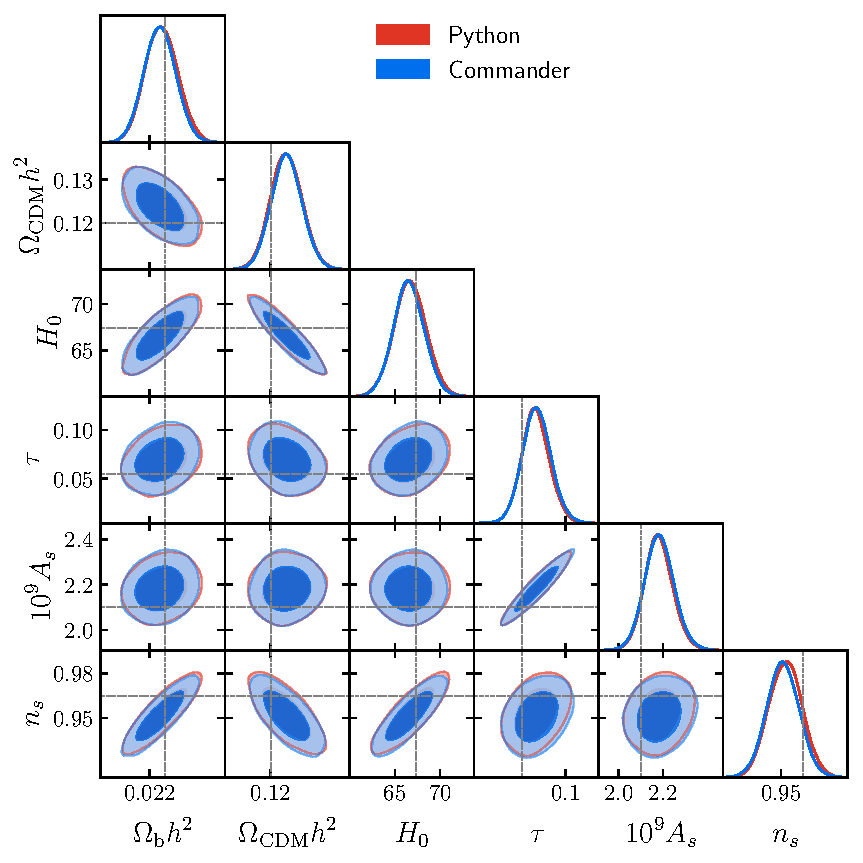
\includegraphics[width=\linewidth]{figures/dist_posterior_no_mask.pdf}
	\caption{\label{fig:nomask}Parameter estimation on a CMB realization with isotropic noise. We use $N_{\mathrm{side}}=512$ and the beam convolve using the beam window functions of 70\,GHz band of Planck. No mask is applied.}
\end{figure}
\begin{figure}
	\centering
	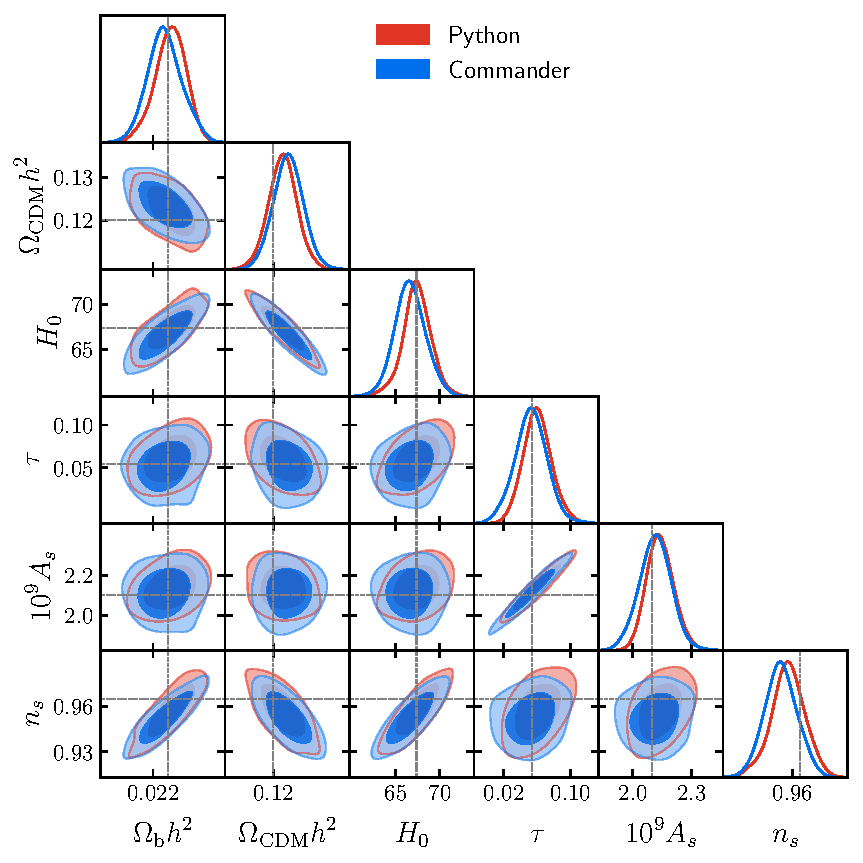
\includegraphics[width=\linewidth]{figures/dist_posterior_10_mask.pdf}
	\caption{Cosmological parameter estimation on same simulation as in Fig.~\ref{fig:nomask} but a constant latitude mask is applied so that the sky fraction is 90\%.}
\end{figure}
\begin{figure}
	\centering
	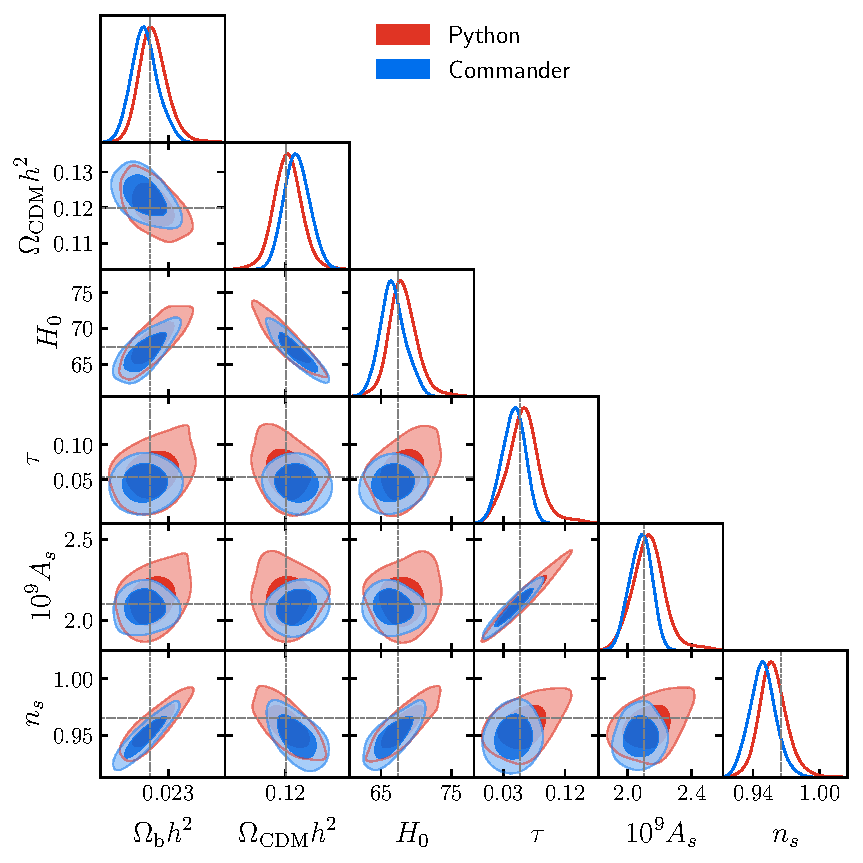
\includegraphics[width=\linewidth]{figures/dist_posterior_20_mask.pdf}
	\caption{Cosmological parameter estimation on same simulation as in Fig.~\ref{fig:nomask} but a constant latitude mask is applied so that the sky fraction is 80\%.}
\end{figure}

\section{Conclusions}
\label{sec:conclusions}

We have shown that the algorithm presented in \cite{racine:2016} works well in the Commander framework for anisotropic noise and mask.

\bibliographystyle{../common/aa}

\bibliography{../common/Planck_bib, ../common/BP_bibliography}

\appendix

\section{Analytic expression for a constant latitude mask}
\label{sec:appendix}


The goal of this appendix is to show how we can calculate $N_{\ell m, \ell' m'}^{-1}$ exactly for a constant latitude mask and uniform noise, and how this makes the map making equation computationally faster to solve. The noise can be written as this in pixel space:
$$
\left(N^{-1} \right)_{pp'} = \frac{N_{\mathrm{pix}}}{\sigma^2} \delta_{pp'} H(|\theta(p) -\pi/2|-b).
$$
where $H$ is the Heavyside function, meaning that we mask every pixel $p$ where $|\theta(p) -\pi/2| < b$ for some latitude $b$ in radians. For a masked pixel, $\left(N^{-1} \right)_{pp}=0$ which means that $N_{pp} = \infty$ for that pixel, as we want.

We then want to calculate $\left(N^{-1}\right)_{\ell m\ell'm'}$. Using that
$$
\left(N^{-1}\right)_{pp'} = \sum_{\ell m}\sum_{\ell' m'} \left(N^{-1}\right)_{\ell m, \ell'm'} Y_{\ell m}\left(p\right)Y^*_{\ell' m'}\left(p'\right),
$$
where $Y_{\ell m}\left(p\right) = Y_{\ell m}\left(\hat{n}(p)\right)$ and $\hat{n}(p)$ are the spherical coordinates for pixel $p$.

Transforming this to spherical harmonics space gives us
\begin{align}
\nonumber
\left(N^{-1}\right)_{\ell m, \ell' m'} &= \sum_{p p'}\left(N^{-1}\right)_{pp'}Y^{*}_{\ell m}(p)Y_{\ell' m'}(p')\\
\nonumber
&= \frac{N_{\mathrm{pix}}}{\sigma^2}\sum_{p p'} Y^{*}_{\ell m}(p)Y_{\ell' m'}(p') \delta_{pp'} H(|\theta -\pi/2|-b)\\
\nonumber
&= \frac{N_{\mathrm{pix}}}{\sigma^2}\sum_{p } Y^{*}_{\ell m}(p)Y_{\ell' m'}(p) H(|\theta -\pi/2|-b)\\
&= \frac{N_{\mathrm{pix}}}{\sigma^2}\sum_p \Tilde{Y}_{\ell m}\Tilde{Y}_{\ell' m'} e^{-i(m-m')\phi} H(|\theta -\pi/2|-b).
\end{align}
Here, we used that $Y_{\ell m}(p) = \tilde{Y}_{\ell m} e^{im\phi}$ where it is implied that $\tilde{Y}_{\ell m}=\tilde{Y}_{\ell m}(\theta)$, and $\theta$ and $\phi$ are functions of $p$.

We now take the limit where there is an infinite amount of pixels with equal surface area each. In this limit, we change the sum into an integration where we account for the number of pixels per area element
\begin{equation}
\sum_p \rightarrow \frac{N_{\mathrm{pix}}}{4\pi}\int d\Omega  = \frac{N_{\mathrm{pix}}}{4\pi}\int_{0}^{2\pi} d\phi \int_{0}^{\pi} d\theta \sin(\theta).
\end{equation}
This gives us in spherical coordinates
\begin{align}
\nonumber
\left(N^{-1}\right)_{\ell m, \ell' m'} &= \frac{N_{\mathrm{pix}}^2}{4\pi \sigma^2}\int_{0}^{2\pi} d\phi \int_{0}^{\pi} d\theta \sin(\theta)\tilde{Y}_{\ell m}  \tilde{Y}_{\ell' m'}  e^{-i(m-m')\phi}
\\
\nonumber
&\cdot H(|\theta -\pi/2|-b)\\
\nonumber
&= \frac{N_{\mathrm{pix}}^2}{2\sigma^2} \delta_{mm'}\int_{0}^{\pi} d\theta \sin(\theta)\tilde{Y}_{\ell m}  \tilde{Y}_{\ell' m'} H(|\theta -\pi/2|-b)\\
\nonumber
&= \frac{N_{\mathrm{pix}}^2}{2\sigma^2} \delta_{mm'}\\
&\cdot \left(\int_{0}^{\pi/2-b} d\theta \sin(\theta) \tilde{Y}_{\ell m}  \tilde{Y}_{\ell' m'}+\int_{\pi/2+b}^{\pi} d\theta \sin(\theta)\tilde{Y}_{\ell m}  \tilde{Y}_{\ell' m'}\right).
\end{align}
Writing the above equation in terms of Legendre polynomials $P_{\ell m}(\cos(\theta)))$, we have
$\Tilde{Y}_{\ell m} = \Delta_{\ell m}P_{\ell m}(\cos(\theta)))$, where ${\Delta_{\ell m}=(-1)^m \sqrt{\frac{2\ell+1}{4\pi}\frac{(\ell - m)!}{(\ell+m)!}}}$.
 Writing $x=\cos(\theta)$, we know that Legendre polynomials $P_{\ell m}(x)$ are either symmetric or antisymmetric in $x\rightarrow-x$. $P_{\ell m}(x)$ is symmetric in $x \rightarrow -x$ when $\ell+m$ = even and antisymmetric when $\ell+m$ = odd. Since $m=m'$, an important feature is that the two integrals cancel each other if $\ell+\ell' =$ odd. We therefore only get non-zero elements when $\ell + \ell' =$ even, for which the two integrals are equal. Hence, for $\ell + \ell'=$ even, we get
\begin{align}
\nonumber
\left(N^{-1}\right)_{\ell m, \ell' m'} &= \frac{N_{\mathrm{pix}}^2}{\sigma^2} \delta_{mm'}\int_{0}^{\pi/2-b} d\theta \sin(\theta)\Tilde{Y}_{\ell m}(\theta)\Tilde{Y}_{\ell' m'}(\theta)\\
\label{eq:finished_n_inv}
&=\frac{N_{\mathrm{pix}}^2}{\sigma^2} \delta_{mm'}\int_{\sin(b)}^{1} dx \, \Tilde{Y}_{\ell m}(\arccos(x)) \Tilde{Y}_{\ell' m}(\arccos(x)).
\end{align}
This integral can be solved numerically by gridding $x$ and the spherical harmonics without phase can be calculated in Python using a library like ...

Since the masks used for this work are $\sin(b)\geq 0.2$, we require much fewer grid points for $x$ if we use the following identity for $\ell+\ell' = $ even:
\begin{align}
&\delta_{mm'} \int_{\sin(b)}^{1} dx \, \Tilde{Y}_{\ell m}(\arccos(x)) \Tilde{Y}_{\ell' m}(\arccos(x)) = \\
\frac{1}{4\pi}\delta_{\ell \ell'}\delta_{m m'} - &\delta_{mm'} \int_{0}^{\sin(b)} dx \, \Tilde{Y}_{\ell m}(\arccos(x)) \Tilde{Y}_{\ell' m}(\arccos(x)),
\end{align}
which comes from the orthonormality condition for spherical harmonics. We now only need to grid $x$ in the interval $0\leq x \leq \sin(b) \leq 0.2$ for this work.

Since our expression for $N^{-1}_{\ell m, \ell' m'}$ has a $\delta_{m m'}$, we can create an $\ell_{\textrm{max}}$ number of matrices, one for each $\ell_{\mathrm{max}}\geq m \geq 0$. And then solve the map-making equation for each matrix equation $m$.

To show how this works in matrix multiplication notation, imagine multiplying the matrix $\textbf{N}^{-1} = N^{-1}_{\ell m, \ell' m'}$ with the vector $\textbf{b} = b_{\ell m}$
\begin{align}
\textbf{N}^{-1} \cdot \textbf{b} &= \sum_{\ell' m'}\left(N^{-1}\right)_{\ell m, \ell' m'}b_{\ell' m'} = \sum_{\ell'}\left(N^{-1}\right)_{\ell m, \ell' m}b_{\ell' m}\\
&= \sum_{\ell' }\left(N^{-1}\right)^{(m)}_{\ell, \ell'}b^{(m)}_{\ell'}.
\end{align}
So to solve the map-making equation, we get a matrix equation for each $\ell_{\mathrm{max}}\geq m \geq 0$. This gives us $\ell_{\textrm{max}}$ number of matrix equations where the dimensions of the matrices are maximal $\ell_{\textrm{max}} \times \ell_{\textrm{max}}$. This is numerically much quicker than inverting the full $(\ell_{\textrm{max}})^2 \times (\ell_{\textrm{max}})^2$ matrix once.


\end{document}